\documentclass[]{article}
\usepackage[T1]{fontenc}
\usepackage[pdftex]{graphicx}
\graphicspath{ {./img/} }
\usepackage{graphicx}
%opening
\title{Book shop}
\author{Kacper Wójcik, Marcin Stefaonwicz, Paweł Nowak}

\begin{document}

\maketitle

\begin{abstract}
	Book shop jest projektem sklepu internetowego z książkami. Głównym założeniem było stworzenie platformy przy użyciu Spring Boota z Mavenem, która pomoże użytkownikom w prowadzeniu sklepu internetowego.

\end{abstract}
\newpage

\section{Projekt systemu}
System składa się z kilku dockerowych kontenerów stworzonych przy użyciu Docker Compose takich jak:
\begin{itemize}
	\item Spring App
	\item React
	\item PostgreSQL
\end{itemize}
\begin{figure}[h]
	\centering
	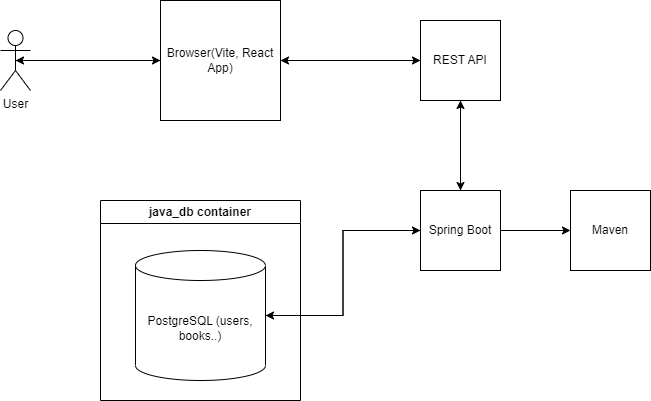
\includegraphics[scale=0.45]{ogolny_projekt.png}
	\caption{Ogólny projekt systemu}
\end{figure}
\subsection{Spring App}
\subsection{React}
\subsection{PostgreSQL}
Ostatni kontener przechowuje i pozwala zarządzać bazą danych PostgreSQL. Została wystawiona na port 5433, aby umożliwić wymianę danych między kontenerami, a jej zabezpieczenia np. możliwość stworzenia indywidualnych kont, oraz haseł pozwala zachować nam względne bezpieczeństwo. PostgreSQL został wybrany ze względu na jego popularność, szybkość działania, oraz to, że jest oparty na modelu relacyjnym.
Baza danych zawiera w aktualnej formie 6 tabel, którymi są:
\begin{itemize}
	\item Users
	\item Authors
	\item Orders
	\item OrderDetails
	\item Books
	\item BookCategories
\end{itemize}
\begin{figure}[h]
	\centering
	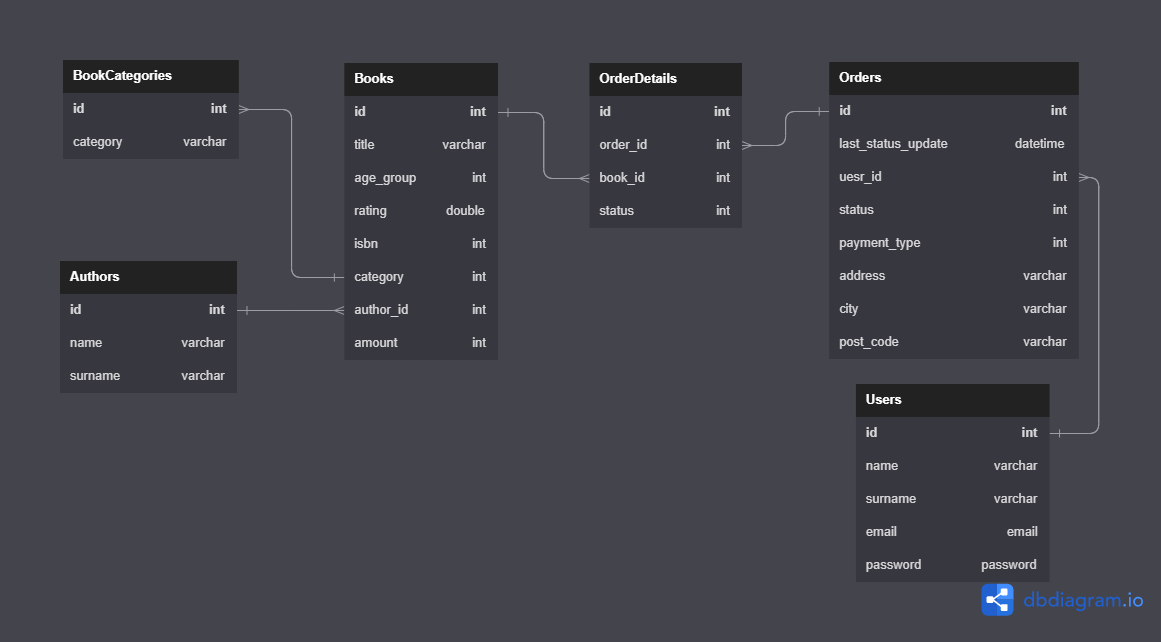
\includegraphics[scale=0.35]{../../DbDiagram.png}
	\caption{Projekt bazy danych}
\end{figure}

\end{document}
